
%%%%%%%%%%%%%%%%%%%%%%%%%%%%%%%%  ejemplo.tex %%%%%%%%%%%%%%%%%%%%%%%%%%%%%%%

%%%%% Fichero de ejemplo LaTeX que ilustra el uso de la Hoja de Estilo %%%%%%
%%%%% Jornadas.cls para las XXII Jornadas de Paralelismo.              %%%%%%

\documentclass[twocolumn,twoside]{Jornadas}
\usepackage{fontspec}
\usepackage{xunicode}
\usepackage{xltxtra}
\usepackage{graphicx}
\graphicspath{{imgs/}}

\usepackage{listings}
\usepackage{color}
\lstloadlanguages{Python}
\lstset{
  language=Python,                      % C,Fortran,XML
  basicstyle=\scriptsize,               % Listados en small
  keywordstyle=\color{red},             % Palabras clave en rojo
  identifierstyle=\ttfamily,
  escapeinside={(*@}{@*)},
  commentstyle=\color{blue},            % comentarios en azul
  stringstyle=\color{green},            % cadenas en verde
  showstringspaces=false,
  frame=tb,
  captionpos=t,
  belowcaptionskip=12pt,
  stepnumber=2,                                         % Opciones de lineas y etiquetas
  numberstyle=\scriptsize,
  numbersep=5pt,
  tabsize=1
}


%%%%%%%%%%%%%%%%%%%%%%%%%%%%%%%%%%%%%%%%%%%%

\begin{document}


\title{Experiencias con Python y CUDA en Computación de Altas Prestaciones}

\author{Sergio Armas, %
     Lionel Mena, %
     Alejandro Samarín,\\*% 
     Vicente Blanco %
     \thanks{Dpto. Estadística, I.O. y Computación, Univ. La Laguna, e-mail: {\tt vblanco@ull.es}}, %
     Alberto Morales y % 
     Francisco Almeida
}

\maketitle
% Oculta las cabeceras y los números de página.
% Ambos elemetos se añadirán durante la edición de las actas completas.
\markboth{}{}
\pagestyle{empty} 
\thispagestyle{empty} % Oculta el número de la primera página

\begin{abstract}
La computación paralela no ha cesado de explorar nuevos horizontes con el objetivo de obtener mejoras tangibles de rendimiento en la ejecución de algoritmos de toda clase. Si bien durante muchos años se ha seguido el camino tradicional de innovar en la arquitectura de las CPU y crear software que aproveche esos beneficios, la consolidación de la que están disfrutando en la última década los dispositivos gráficos como hardware de cómputo general es difícil de ignorar. Este cambio de paradigma trae consigo nuevas formas de programar, nuevas herramientas y por supuesto, nuevos desafíos. El hecho de que el lenguaje C y sus derivados sean la \emph{lingua franca} de este tipo de programación no debería sorprender a propios ni a extraños, pero otros lenguajes se van haciendo hueco poco a poco: es el caso de Python, que gracias al \emph{wrapper} PyCUDA \cite{DBLP:journals/corr/abs-0911-3456} es capaz de ofrecer al programador el acceso a la computación de altas prestaciones sobre dispositivos gráficos sin renunciar a la comodidad y el dinamismo de este lenguaje. El propósito de este artículo es comprobar las facilidades que promete PyCUDA así como su rendimiento frente a problemas reales.
\end{abstract}

\begin{keywords}
Python, CUDA, PyCUDA
\end{keywords}

\section{Introducción}

La capacidad de cómputo de las unidades de procesamiento gráfico (GPU) ha alcanzado en los últimos años un desarrollo notable que ha crecido de manera paralela a un fuerte incremento en la producción y demanda de dispositivos que las integran, tales como smartphones, tablets, etc., además de seguir presentes en tarjetas gráficas o placas base con cada vez más relevancia. Precisamente, dicho aumento de potencia ha comenzado a hacer atractivo su empleo para la manipulación de cantidades masivas de datos en ámbitos ajenos al del video tales como criptología, biología computacional, cálculo científico etc., que, por su naturaleza paralela, son susceptibles de ejecutarse con más eficiencia, incluso, que en una CPU tradicional. Esta técnica de usar la GPU en aplicaciones que tradicionalmente se habían ejecutado en CPU recibe el nombre de GPGPU (General-purpose computing on graphics processing units).

\vspace{5 mm}

A pesar de que existen diversos fabricantes especializados en dispositivos gráficos que ofrecen algún tipo de \emph{framework} para desarrollo de aplicaciones paralelas sobre GPGPU, e incluso alternativas más generales como OpenCL \cite{opencl}, NVIDIA es probablemente el fabricante especializado que más ha apostado por este enfoque. Prácticamente desde los albores de la computación de este tipo, han ido desarrollando un modelo de programación denominado CUDA (Compute Unified Device Architecture) \cite{aboutcuda}, que permite al programador ejecutar algoritmos casi arbitrarios en sus GPU. El lenguaje de programación diseñado para ello es una variación de C que contiene extensiones para trabajar con la GPU, amén de ciertas restricciones (no permite recursividad ni punteros a funciones, solo permite números en precisión simple en la mayoría de tarjetas lanzadas al mercado hasta ahora, etc.).

\vspace{5 mm}

El término anglosajón \emph{wrapper} se emplea en computación para designar, a grandes rasgos, un tipo de software que añade una capa de código para traducir de una interfaz existente a otra, generalmente con la finalidad de ganar portabilidad, sencillez o compatibilidad. PyCUDA, que ha sido desarrollado por Andreas Klöckner \footnote[2]{Courant Institute of Mathematical Sciences - New York University - {\tt http://mathema.tician.de/aboutme}}, es un ejemplo de esto: ejerce la función de interfaz en Python para las funciones nativas escritas en C que proporciona la SDK de NVIDIA. La principal ventaja que representa la utilización de PyCUDA en el desarrollo, en contraposición al uso de las funciones propias de NVIDIA bajo C/C++, es sin duda la comodidad. PyCUDA permite abstraer, por ejemplo, de todo lo relacionado con la reserva y liberación de memoria en el dispositivo, lo cual hubiera representado una carga adicional de trabajo destacable en la versión C/C++. En este artículo se analizará si las ventajas de utilizar un lenguaje interpretado de muy alto nivel para ejecutar algoritmos en una GPU compensa la menor velocidad inherente a los lenguajes interpretados.
Para ello, se abordan dos problemas característicos: el producto matricial y la detección de movimiento.

\ldots utilizando PyCUDA~\cite{DBLP:journals/corr/abs-0911-3456}

y una gráfica \ref{fig:Fermi}

\begin{figure}
	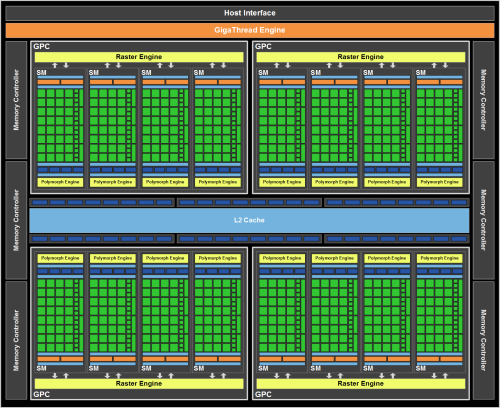
\includegraphics[width=.45\textwidth]{block_diagram_Fermi}
	\caption{\label{fig:Fermi} Diagrama de bloques de una GPU Tesla M2070 (Fermi)}
\end{figure}

y un código \ref{code:filter}

\section{Ejecución de un kernel con PyCUDA}

No existe una única manera de ejecutar un algoritmo en un dispositivo con PyCUDA y, por supuesto, no todas resultan igual de eficientes. A continuación, se mostrará una sencilla secuencia de instrucciones que ilustran de manera bastante exacta el nivel de abstracción que puede llegar a alcanzarse sin menoscabo de la eficiencia.

En primer lugar, se importan los mínimos paquetes necesarios para el funcionamiento de PyCUDA:

\begin{verbatim}
import pycuda.autoinit
import pycuda.driver as cuda
from pycuda.compiler import SourceModule
\end{verbatim}

Conviene hacer notar que aunque {\tt pycuda.autoinit} se encarga de inicializar el dispositivo (seleccionando el de mayor capacidad de cómputo si hay más de uno), así como de crear un contexto automáticamente, ambos aspectos pueden ser configurados manualmente.

El siguiente paso consiste en cargar en memoria los datos que se desean procesar. En este punto, resulta muy aconsejable el uso del paquete {\tt NumPy} de la librería {\tt SciPy}, pues está provisto del potente tipo de dato {\tt numpy.array}, que facilita la preparación y manipulación de los datos. En este ejemplo, consideraremos dos arrays aleatorios \emph{a} y \emph{b}, cuyas componentes se restan dos a dos sobreescribiendo \emph{b} con el resultado.

\begin{verbatim}
import numpy as np
a = np.random.randn(16)
b = np.random.randn(16)
\end{verbatim}

Aunque las más recientes GPU soportan números en coma flotante de doble precisión, la mayoría de los dispositivos disponibles actualmente solo soportan precisión simple, por lo que se impone la siguiente conversión de tipos:

\begin{verbatim}
a.astype(np.float32)
b.astype(np.float32)
\end{verbatim}

Una vez cargados los datos en memoria, los siguientes pasos son transferirlos al dispositivo y ejecutar el kernel. Con PyCUDA, ambos pasos pueden concentrar en uno solo, porque en la propia llamada al kernel puede estar implícita la transferencia de los datos a la memoria del dispositivo si se hace uso de la clase {\tt ArgumentHandler} disponible en {\tt pycuda.driver}, la cual está preparada para trabajar con arrays numpy como argumentos de entrada/salida.

\begin{verbatim}
kernel = SourceModule("""
  __global__ void name(float *a, float *b) {
    int idx = threadIdx.x;
    b[idx] = b[idx] - a[idx];
  }
  """)
f = kernel.get_function("name")
f(cuda.In(a), cuda.InOut(b), block=(16,16,1))
\end{verbatim}

\section{Producto matricial}

La manera tradicional de abordar la multiplicación de matrices pasa por ejecutar un algoritmo secuencial de complejidad casi cúbica en las mejores implementaciones. Su versión paralela, en cambio, permite el cálculo simultáneo de las filas de la primera matriz multiplicando con la correspondiente columna de la segunda para formar el resultado.

PyCUBLAS o nuestros matrixmult?

\section{Producto matricial}

\section{Detección de movimiento}

El algoritmo de detección de movimiento consiste, en su versión más simple, en la aplicación de tres filtros (por este orden: Difference, Threshold y Erosion) a cada par de fotogramas de la secuencia que se analiza. Como resulta fácil constatar, a poco que tratemos la detección de movimiento en un video de pocos segundos de duración, la carga computacional será bastante elevada.

En el anexo de este artículo se proporciona el paquete Filters, que se estructura, esencialmente, en torno a dos clases: CUDAHandler, concebida para abstraer aún mas la comunicación con el dispositivo (informalmente, se podría considerarla como un wrapper del propio PyCUDA), y Filter, clase abstracta cuyas clases hijas se corresponden con cada uno de los filtros implementados.

Además, la clase MotionDetector se encarga de realizar la detección en sí haciendo uso del paquete antes mencionado, y la clase VideoHandler abstrae la manipulación de las operaciones de gestión de video.

%\lstinputlisting[%
%   float=t,
%   caption={Codigo de filtros en Python},
%   label={code:filter} 
%   ]%
%   {code/filter.py}

\bibliographystyle{Jornadas}
\bibliography{pycuda}

\end{document}

